\documentclass[11pt,a4paper]{article}
\usepackage[margin=25mm]{geometry}
\usepackage{amsmath,amssymb,booktabs,array,xcolor,tikz,hyperref}
\usepackage[T1]{fontenc}
\usepackage{lmodern}
\hypersetup{colorlinks=true,linkcolor=blue,urlcolor=blue}
\setlength{\parindent}{0pt}
\setlength{\parskip}{6pt}
\newcommand{\vect}[1]{\mathbf{#1}}
\title{Rainfall tomography in Giuli et al. (1991)\\\large An explanatory guide to the model, regularization, and solver}
\author{Method notes based on the original paper}
\date{29 September 2026}
\begin{document}
\maketitle
\begin{abstract}
Giuli et al. reconstruct a spatial field of microwave specific attenuation from a small number of path-integrated attenuation measurements, then convert that field to rainfall. This intermediate variable makes their inverse problem a convex quadratic optimization problem. These notes explain the basis functions, measurement weights, regularization, and iterative solution. They also distinguish prescribed spatial structure from simulation-based parameter tuning and flag an inconsistency in the paper's parameter labels.
\end{abstract}
\section{The central idea}
A microwave link provides one number: the total rain-induced signal loss along its path. That number does not reveal where along the path the rain occurred. Several intersecting links provide complementary information, but usually still too little to determine a detailed field uniquely.

The method follows this chain:
\[
\boxed{\text{Link attenuations }\vect p}
\ \longrightarrow\ 
\boxed{\text{Attenuation field }\widehat K(x,y)}
\ \longrightarrow\ 
\boxed{\text{Rain field }\widehat R(x,y)}.
\]
Specific attenuation $K$ means loss per unit distance (dB/km); total link attenuation $p_m$ means accumulated loss (dB). Their relationship is a line integral:
\begin{equation}
p_m=\int_{\text{link }m}K(x,y)\,d\ell.
\end{equation}
Here $\ell$ measures distance along the link. More explicitly, with link length $L_m$ and path coordinates $(x_m(\ell),y_m(\ell))$,
\[
p_m=\int_0^{L_m}K(x_m(\ell),y_m(\ell))\,d\ell.
\]
The location $(x,y)$ therefore varies as we move along the link; it is not a separate integration variable.

\textbf{Why is this linear in $K$?} Giuli assumes that every link uses the same
rainfall-to-attenuation law. In the simulation all links use wavelength
$0.86$~cm (about $35$~GHz), with the common relation
\[
K(x,y)=0.221R(x,y)^{1.04}.
\]
Thus there is one shared specific-attenuation field $K$ for all links, and
each link simply integrates that same field along a different path. If links
had different exponents, $K_m=a_mR^{b_m}$ would be link-dependent; one shared
$K$ would no longer produce the simple linear model $\vect p=\vect A\vect k$.
Different prefactors with a common exponent could be absorbed into link
weights, but different exponents make the forward model nonlinear in a chosen
reference attenuation field.

\textbf{What was measured in this paper?} The reported experiment is a simulation. Rainfall is generated from a stochastic model, converted to attenuation, integrated along hypothetical links, and corrupted with simulated errors. The proposed dedicated network has six transmitters, two receivers, and twelve links. It is not an experiment using deployed commercial or laboratory links.
\section{Notation: what is known and what is unknown?}
\begin{center}
\begin{tabular}{p{24mm}p{104mm}}
\toprule
Symbol & Meaning \\
\midrule
$(x,y)$ & A physical location in the reconstruction area.\\
$n=1,\ldots,N$ & Index selecting a basis function/grid center.\\
$m=1,\ldots,M$ & Index selecting a microwave link.\\
$b_n(x,y)$ & Known, dimensionless spatial shape centered at grid location $n$.\\
$k_n$ & Unknown multiplier of that shape; units dB/km.\\
$p_m$ & Observed (synthetic in the experiment) total attenuation on link $m$; units dB.\\
$A_{mn}$ & Known integral of shape $n$ along link $m$; units km.\\
\bottomrule
\end{tabular}
\end{center}
An index and a coordinate do different jobs: $b_2(3,7)$ means ``evaluate basis function number 2 at the location $(3,7)$.'' It does not mean that basis function 2 exists only at that location.
\section{Representing a field with overlapping tents}
The specific-attenuation field is approximated by
\begin{equation}
\widehat K(x,y)=\sum_{n=1}^N k_n b_n(x,y).
\end{equation}
There is one basis function per grid cell, centered at $(r_n,s_n)$. If adjacent centers are separated by $\Delta$, define
\[
\Lambda(u)=\max(1-|u|,0),\qquad
b_n(x,y)=\Lambda\!\left(\frac{x-r_n}{\Delta}\right)
\Lambda\!\left(\frac{y-s_n}{\Delta}\right).
\]
The symbol $s_n$ here is a center's $y$ coordinate, not distance along a link. The shape equals one at its own center and zero at every other grid center. Its support is a square of side $2\Delta$, so it overlaps neighboring shapes. The shape is fixed; only its coefficient is reconstructed.

\begin{center}
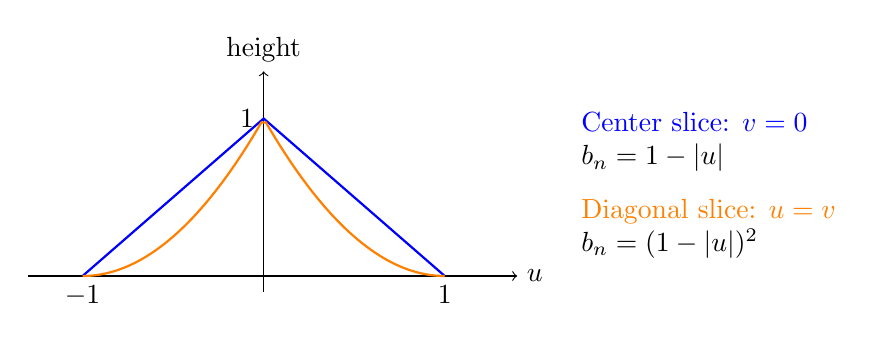
\begin{tikzpicture}[x=2.3cm,y=2.0cm]
\draw[->] (-1.3,0)--(1.4,0) node[right] {$u$};
\draw[->] (0,-.1)--(0,1.3) node[above] {height};
\draw[thick,blue] (-1,0)--(0,1)--(1,0);
\draw[thick,orange,domain=-1:1,samples=80] plot (\x,{(1-abs(\x))^2});
\node[below] at (-1,0) {$-1$};\node[below] at (1,0) {$1$};
\node[left] at (0,1) {$1$};
\node[align=left,anchor=west] at (1.7,.85) {\textcolor{blue}{Center slice: $v=0$}\\$b_n=1-|u|$};
\node[align=left,anchor=west] at (1.7,.3) {\textcolor{orange}{Diagonal slice: $u=v$}\\$b_n=(1-|u|)^2$};
\end{tikzpicture}
\end{center}
Here $u=(x-r_n)/\Delta$ and $v=(y-s_n)/\Delta$. The surface resembles a tent or pyramid, but it is bilinear in each quadrant, rather than a pyramid with flat triangular faces. The diagonal cross-section is curved.

At a grid center, $\widehat K(r_n,s_n)=k_n$. Thus $HW$ such functions on an $H\times W$ grid give $HW$ independent coefficients and can match arbitrary values at those centers. Between centers, bilinear interpolation fixes the field. Arbitrary sub-grid detail cannot be represented; near the outer support boundary the representation also imposes a taper toward zero.
\section{Why the matrix weights are line integrals}
Substituting the field expansion into the measurement model gives
\begin{align}
\widehat p_m
&=\int_{\text{link }m}\sum_n k_n b_n(x,y)\,d\ell\\
&=\sum_n k_n\underbrace{\int_{\text{link }m}b_n(x,y)\,d\ell}_{A_{mn}}.
\end{align}
Each $k_n$ is constant during integration. Therefore the forward model is
\begin{equation}
\vect p=\vect A\vect k+\vect e,
\end{equation}
where $\vect e$ accounts for errors, including measurement and representation errors.

\textbf{Geometric interpretation.} A link missing a tent has weight zero. A link crossing its low edge picks up a small integral. A link passing through a taller part picks up a larger integral, for comparable path lengths. These are consequences of geometry, not fitted statistical weights.

\textbf{Example.} A horizontal link crossing the entire tent through its center sees a triangular profile of base $2\Delta$ and height one. Hence $A_{mn}=\Delta$. If $\Delta=1$ km and $k_n=3$ dB/km, that shape contributes $3$ dB to the link. Crossing the full support at a vertical offset $\Delta/2$ halves the weight and contributes $1.5$ dB instead.

The units agree: $A_{mn}k_n$ has units $\text{km}\times\text{dB/km}=\text{dB}$. Summing over $n$ gives the predicted total loss for link $m$.
\section{Why regularization is necessary}
The simulation uses $N=25$ coefficients but only $M=12$ links, so $\vect A$ is $12\times25$ and its rank is at most 12. Independent basis functions do not imply enough independent observations. Many coefficient vectors can produce the same link predictions.

Regularization selects a preferred solution by imposing small magnitude and local smoothness. It does not create new observations or guarantee recovery of the true field.
\section{The exact quadratic objective}
Following the labels in the paper's Eq.~(19), p.~1330, the objective is
\begin{equation}\label{eq:obj}
J(\vect k)=\frac12\vect k^\top(\vect I+b_0\vect B)\vect k
+\frac{a_0}{2}\|\vect p-\vect A\vect k\|_2^2.
\end{equation}
The algorithm also enforces $\vect k\geq0$. The spatial matrix satisfies
\[
\vect k^\top\vect B\vect k
=\sum_{i\in S}\left(k_i-\frac18\sum_{j\in S_i}k_j\right)^2,
\]
where $S$ contains interior grid cells and $S_i$ contains the eight neighbors of cell $i$. Thus the three terms mean:
\[
\boxed{
J(\vect k)=
\underbrace{\frac12\|\vect k\|_2^2}_{\text{prefer smaller attenuation}}
+\underbrace{\frac{b_0}{2}\sum_{i\in S}
\left(k_i-\frac18\sum_{j\in S_i}k_j\right)^2}_{\text{prefer local smoothness}}
+\underbrace{\frac{a_0}{2}\|\vect p-\vect A\vect k\|_2^2}_{\text{fit measured link attenuation}}
}
\]
This is the same objective in a more readable form. The first term is a
small-magnitude preference, the second penalizes a cell's departure from the
mean of its eight neighbors, and the third penalizes disagreement between
the predicted and observed path attenuations. The data term prevents the
zero field from being optimal when the links observe rain.
\begin{enumerate}
\item $\tfrac12\|\vect k\|^2$: discourage large attenuation coefficients. Alone this favors zero. The paper motivates it through a variance criterion, replacing variance by squared norm under a constant-mean assumption; the final objective uses the norm.
\item $\tfrac{b_0}{2}\vect k^\top\vect B\vect k$: discourage departure from the local neighbor average. This is a fixed spatial smoothness assumption.
\item $\tfrac{a_0}{2}\|\vect p-\vect A\vect k\|^2$: discourage disagreement with the measured link losses.
\end{enumerate}
For $a_0>0$, division by $a_0$ leaves the minimizer unchanged. Relative to measurement fit, the magnitude and smoothness penalties therefore have strengths $1/a_0$ and $b_0/a_0$.

\textbf{Do they learn a covariance?} No empirical spatial covariance is estimated for $\vect B$: Eqs.~(14)--(18) construct it from the fixed eight-neighbor stencil. However, the scalar parameters are tuned in simulations. Page 1337 reports settings $a_0=2.5$, $b_0=15$ and a progressive parameter search. This is not documented as a systematic two-dimensional grid search or a separate training/test procedure. Equation (30) also uses current link measurements to initialize all coefficients to their mean path-specific attenuation; that is initialization, not covariance learning.

\textbf{Important notation inconsistency.} The discussion on p.~1337 assigns the roles of $a_0$ and $b_0$ oppositely to Eq.~(19). Figure 11 discusses $a_0=0$ as removing a correlation constraint, whereas literal substitution into Eq.~(19) removes measurement fit. The objective and solver in these notes follow Eqs.~(19)--(20); the later numerical parameter labels should not be treated as unambiguous implementation specifications.
\section{Convexity and the iterative solver}
For fixed nonnegative weights,
\[
\nabla J(\vect k)=(\vect I+b_0\vect B)\vect k
+a_0\vect A^\top(\vect A\vect k-\vect p),\qquad
\vect H=\nabla^2J=\vect I+b_0\vect B+a_0\vect A^\top\vect A.
\]
Both $\vect B$ and $\vect A^\top\vect A$ are positive semidefinite because their quadratic forms are sums of squares. The identity makes $\vect H$ positive definite: the objective is strictly convex, with a unique minimizer. Nonnegativity is a convex constraint and preserves uniqueness.

Equation (20) gives a fixed-step gradient iteration, attributed to Herman and Lent (1976b). With the clipping described on p.~1333, it is what we now call projected gradient descent:
\begin{equation}
\vect k^{(\ell+1)}=\left[\vect k^{(\ell)}-\frac1\gamma\nabla J(\vect k^{(\ell)})\right]_+.
\end{equation}
The notation $[\cdot]_+$ means set negative components to zero. The paper sets
\[
\gamma=\frac{\mu_{\max}+\mu_{\min}}2,
\]
using the extreme eigenvalues of $\vect H$ (Eq.~21). Consequently the step is $2/(\mu_{\max}+\mu_{\min})$. For this positive-definite quadratic it lies within the standard convergence interval $(0,2/\mu_{\max})$.

An implementation consistent with the equations is:
\begin{enumerate}
\item Construct $\vect A$ from the fixed link geometry and basis functions; construct $\vect B$ from grid neighbors.
\item Choose nonnegative weights, taking care with the paper's labeling inconsistency; compute the step size.
\item At each observation time, initialize each coefficient to $M^{-1}\sum_m p_m/L_m$, as in Eq.~(30).
\item Repeat the gradient update and nonnegativity projection until a chosen convergence tolerance is met. This tolerance is an implementation choice here, not a quoted paper setting.
\item Evaluate the basis expansion and convert attenuation to rainfall.
\end{enumerate}
\section{Why nonlinear rainfall physics does not break convexity}
The power law is $K=aR^b$, where these physical coefficients $a,b$ are distinct from optimization weights $a_0,b_0$. The simulation uses
\[
K=0.221R^{1.04}
\]
for wavelength $0.86$ cm, attributed to Atlas and Ulbrich (1977), not to an ITU standard (Eqs.~27--28).

The inverse optimization uses $K$ coefficients, for which path integration is linear. Only afterward does it apply
\[
\widehat R(x,y)=\left(\frac{\widehat K(x,y)}a\right)^{1/b}.
\]
This assumes a known applicable power law. Its nonlinear conversion is not part of the quadratic optimization. Direct optimization over rainfall would generally lose the guarantee of convexity. Moreover, smoothness in attenuation is not exactly the same as a quadratic smoothness penalty in rainfall. The method's shared attenuation field is appropriate to its common-frequency setup; mixed link-specific power laws require additional modeling.

More generally, if link $m$ had its own law
\[
K_m(x,y)=a_mR(x,y)^{b_m},
\]
then choosing a reference field
$K_{\rm ref}=a_0R^{b_0}$ would give
\[
p_m=\int_{\text{link }m}a_m
\left(\frac{K_{\rm ref}(x,y)}{a_0}\right)^{b_m/b_0}d\ell.
\]
This remains linear only when the exponents are common ($b_m=b_0$). Giuli's
linear attenuation reconstruction therefore relies on the common-frequency,
common-law simulation setup.
\section{Where to check the original paper}
\begin{center}
\begin{tabular}{p{25mm}p{100mm}}
\toprule
Printed pages & Content \\
\midrule
1328--1329 & Field expansion, link integrals, matrix model, and basis functions: Eqs.~(4)--(10).\\
1330 & Regularizers, exact objective, gradient iteration, and eigenvalue step: Eqs.~(11)--(21).\\
1331--1333 & Synthetic rainfall, network geometry, error models, initialization, and nonnegativity.\\
1337--1339 & Parameter discussion, notation inconsistency, and Fig.~11.\\
\bottomrule
\end{tabular}
\end{center}
\begin{thebibliography}{1}
\bibitem{giuli}
D. Giuli, A. Toccafondi, G. Biffi Gentili, and A. Freni,
``Tomographic Reconstruction of Rainfall Fields through Microwave Attenuation Measurements,''
\emph{Journal of Applied Meteorology}, vol.~30, no.~9, pp.~1323--1340, 1991.
DOI: \href{https://doi.org/10.1175/1520-0450(1991)030<1323:TRORFT>2.0.CO;2}{10.1175/1520-0450(1991)030\textless1323:TRORFT\textgreater2.0.CO;2}.
\end{thebibliography}
\end{document}
